\documentclass[11pt]{article}

\usepackage[utf8]{inputenc}
\usepackage[T1]{fontenc}
\usepackage{lmodern}
\usepackage{geometry}
\geometry{margin=1in}
\usepackage{amsmath,amssymb,amsfonts,amsthm,mathtools,bm}
\usepackage{physics}
\usepackage{tikz}
\usetikzlibrary{arrows.meta,positioning,calc,decorations.pathmorphing,patterns}
\usepackage{hyperref}
\usepackage{enumitem}
\usepackage{authblk}

\hypersetup{colorlinks=true,linkcolor=blue,citecolor=blue,urlcolor=blue}

\newtheorem{theorem}{Theorem}
\newtheorem{proposition}{Proposition}
\newtheorem{lemma}{Lemma}
\newtheorem{definition}{Definition}
\newtheorem{corollary}{Corollary}
\theoremstyle{remark}
\newtheorem{remark}{Remark}

\title{Hidden Confining Gauge Sectors as Effective Gravitational Fluids}
\author{Author Name}
\affil{Independent Research Draft}
\date{Draft \today}

\begin{document}
\maketitle

\begin{abstract}
Ordinary QCD is strongly coupled but short-ranged after confinement, making it an unlikely direct source of galaxy-scale dark matter or cosmic dark energy. A more viable theoretical direction is a hidden confining gauge sector: a dark non-Abelian field theory coupled weakly or gravitationally to the Standard Model. This paper introduces a minimal effective-fluid framework for such sectors. The central classification theorem shows that thermal excitations of a hidden confining sector behave approximately as radiation above confinement and as matter-like relics below confinement, while dark-energy-like behavior $w\approx-1$ requires an additional vacuum-energy or metastable false-vacuum component. The result grounds the intuitive idea that distributed field energy can gravitate globally, but constrains it sharply: confinement alone is not dark energy. The paper proposes lattice-computable observables and cosmological tests, including equation-of-state data, relic abundance, self-interactions, $\Delta N_{\rm eff}$, and gravitational waves from first-order dark confinement transitions.
\end{abstract}

\tableofcontents

\section{Introduction}

The strong interaction shows that most of the proton mass arises not from bare quark masses but from nonperturbative field energy. This motivates a natural question: could a distributed confining field sector produce gravitational phenomena resembling dark matter or dark energy?

For ordinary QCD, the answer is almost certainly no. QCD is already included in baryonic matter, and its confined excitations are short-ranged. But a hidden copy or cousin of QCD, coupled very weakly to the Standard Model, is a serious dark-sector candidate.

\paragraph{New viewpoint.} This paper introduces hidden confinement as an \emph{effective gravitational fluid}. Instead of asking whether strong force itself creates a new long-range force, we ask whether the stress-energy tensor of a hidden confining sector can generate cosmological components with equations of state matching dark matter, dark radiation, or dark energy.

\section{Literature grounding}

Dark non-Abelian gauge sectors have been studied under names such as dark QCD, hidden Yang--Mills, glueball dark matter, dark baryons, and dark pions. They are motivated by accidental stability, confinement, and the fact that gravitational or portal couplings can populate a dark sector while keeping it hard to detect. Lattice studies of pure Yang--Mills thermodynamics provide nonperturbative input for the equation of state. Cosmological studies constrain hidden sectors through structure formation, self-interaction bounds, $\Delta N_{\rm eff}$, relic abundance, and gravitational-wave signatures of first-order phase transitions.

\section{Model}

Consider a hidden gauge theory with group $SU(N_d)$ and field strength $G^a_{\mu\nu}$:
\begin{equation}
\mathcal L_d=-\frac14 G^a_{\mu\nu}G^{a\mu\nu}+\sum_i\bar q_i(i\not{D}-m_i)q_i-\Lambda_{\rm vac}.
\end{equation}
The sector may couple to the Standard Model only gravitationally, or through suppressed portals. Its stress-energy tensor is
\begin{equation}
T^{(d)}_{\mu\nu}=-\frac{2}{\sqrt{-g}}\frac{\delta S_d}{\delta g^{\mu\nu}}.
\end{equation}
At cosmological scales, isotropy and homogeneity allow an effective perfect-fluid form:
\begin{equation}
T^{(d)\mu}_{\quad\nu}=\mathrm{diag}(-\rho_d,p_d,p_d,p_d),\qquad w_d=\frac{p_d}{\rho_d}.
\end{equation}

\section{Effective equation of state}

We decompose the hidden-sector energy density and pressure as
\begin{align}
\rho_d(T_d) &= \rho_{\rm th}(T_d)+B_d,\\
p_d(T_d) &= p_{\rm th}(T_d)-B_d,
\end{align}
where $T_d$ is the dark-sector temperature and $B_d$ is a vacuum-energy offset or bag constant.

At high temperature in a nearly conformal deconfined phase,
\begin{equation}
\rho_{\rm th}\approx \alpha_d T_d^4,
\qquad
p_{\rm th}\approx \frac13\alpha_d T_d^4.
\end{equation}
At low temperature after confinement, stable nonrelativistic relics satisfy
\begin{equation}
p_{\rm th}\ll \rho_{\rm th},
\qquad w\approx0.
\end{equation}

\begin{figure}[h]
\centering
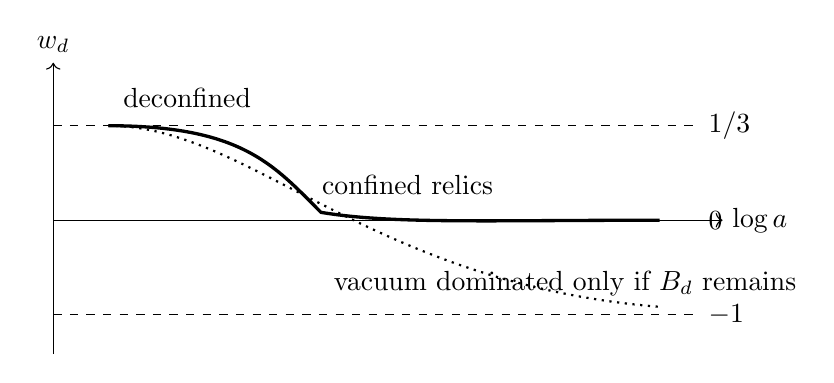
\begin{tikzpicture}[x=1cm,y=1cm]
    \draw[->] (0,0) -- (8.5,0) node[right] {$\log a$};
    \draw[->] (0,-1.7) -- (0,2.0) node[above] {$w_d$};
    \draw[dashed] (0,1.2) -- (8.2,1.2) node[right] {$1/3$};
    \draw[dashed] (0,0) -- (8.2,0) node[right] {$0$};
    \draw[dashed] (0,-1.2) -- (8.2,-1.2) node[right] {$-1$};
    \draw[very thick] (0.7,1.2) .. controls (2.4,1.2) and (2.8,0.7) .. (3.4,0.1) .. controls (4.3,-0.05) and (5.5,0) .. (7.7,0);
    \draw[thick,dotted] (0.7,1.2) .. controls (2.5,1.2) and (4,-0.8) .. (7.7,-1.1);
    \node at (1.7,1.55) {deconfined};
    \node at (4.5,0.45) {confined relics};
    \node at (6.5,-0.8) {vacuum dominated only if $B_d$ remains};
\end{tikzpicture}
\caption{Hidden confinement naturally interpolates between radiation-like and matter-like behavior. Dark-energy-like behavior requires an additional persistent vacuum component.}
\end{figure}

\section{Classification theorem}

\begin{theorem}[Effective-fluid classification]
Consider a homogeneous hidden confining sector with energy density and pressure
\begin{equation}
\rho_d=\rho_{\rm th}+B_d,
\qquad
p_d=p_{\rm th}-B_d,
\end{equation}
where $B_d\ge0$. Suppose the thermal component satisfies $0\le p_{\rm th}\le \rho_{\rm th}/3$. Then:
\begin{enumerate}[label=(\roman*)]
\item if $B_d=0$ and the sector is relativistic, $0\le w_d\le1/3$;
\item if $B_d=0$ and the sector is nonrelativistic, $w_d\approx0$;
\item if $B_d\gg\rho_{\rm th}$, then $w_d\to-1$.
\end{enumerate}
Thus a hidden confining sector does not generically behave as dark energy unless a vacuum-like component dominates.
\end{theorem}

\begin{proof}
The equation-of-state parameter is
\begin{equation}
w_d=\frac{p_{\rm th}-B_d}{\rho_{\rm th}+B_d}.
\end{equation}
If $B_d=0$, then $w_d=p_{\rm th}/\rho_{\rm th}$ and the stated bounds follow. In the nonrelativistic limit $p_{\rm th}/\rho_{\rm th}\ll1$, so $w_d\approx0$. If $B_d\gg\rho_{\rm th},p_{\rm th}$, then numerator and denominator are approximately $-B_d$ and $B_d$, respectively, so $w_d\to-1$.
\end{proof}

\begin{corollary}[Confinement alone is not dark energy]
If the hidden sector contains only ordinary positive-energy thermal excitations and stable bound states, then it can mimic radiation or matter but not a persistent cosmological constant.
\end{corollary}


\subsection{Exact interpolation, acceleration threshold, and sound speed}
The classification can be sharpened when the thermal component has an approximately constant equation of state $p_{\rm th}=w_{\rm th}\rho_{\rm th}$ with $0\le w_{\rm th}\le 1/3$. For $B_d>0$, define
\begin{equation}
 x(a)=\frac{\rho_{\rm th}(a)}{B_d}.
\end{equation}
Then the total equation of state is exactly
\begin{equation}
 w_d(x)=\frac{w_{\rm th}x-1}{x+1}.
 \label{eq:hidden-wx}
\end{equation}

\begin{proposition}[Monotone vacuum interpolation]
If the thermal component is separately conserved and $w_{\rm th}$ is constant, then
\begin{equation}
 x(a)=x_*\left(\frac{a}{a_*}\right)^{-3(1+w_{\rm th})}
\end{equation}
and
\begin{equation}
 \frac{dw_d}{d\ln a}
 =-3(1+w_{\rm th})^2\frac{x}{(1+x)^2}\le0.
 \label{eq:hidden-w-monotone}
\end{equation}
Thus the background equation of state evolves continuously from $w_{\rm th}$ at $x\gg1$ toward $-1$ at $x\ll1$.
\end{proposition}

\begin{proof}
Separate conservation gives $\rho_{\rm th}\propto a^{-3(1+w_{\rm th})}$. Differentiating Eq.~\eqref{eq:hidden-wx} gives
\begin{equation}
 \frac{dw_d}{dx}=\frac{1+w_{\rm th}}{(1+x)^2},
 \qquad
 \frac{dx}{d\ln a}=-3(1+w_{\rm th})x,
\end{equation}
which yields Eq.~\eqref{eq:hidden-w-monotone}.
\end{proof}

The acceleration condition $\rho_d+3p_d<0$ becomes
\begin{equation}
 (1+3w_{\rm th})\rho_{\rm th}<2B_d.
 \label{eq:hidden-acc-threshold}
\end{equation}
Hence a radiation-like thermal sector accelerates only when $B_d>\rho_{\rm th}$, while a matter-like thermal sector accelerates when $B_d>\rho_{\rm th}/2$.

For constant $B_d$ and constant $w_{\rm th}$, the adiabatic background sound speed is
\begin{equation}
 c_a^2\equiv \frac{\dot p_d}{\dot\rho_d}
 =w_{\rm th}c^2,
 \label{eq:hidden-soundspeed}
\end{equation}
provided the vacuum offset does not fluctuate independently. Thus the background value $w_d\to-1$ does not force the perturbation sound speed to approach $-c^2$ or zero; perturbations must be specified separately.

\subsection{Trace-anomaly identity}
The same decomposition gives an exact relation to a lattice observable:
\begin{equation}
 \mathcal I_d(T_d)
 \equiv \rho_d-3p_d
 =\left(\rho_{\rm th}-3p_{\rm th}\right)+4B_d.
 \label{eq:hidden-trace-identity}
\end{equation}
In a nearly conformal deconfined regime where $\rho_{\rm th}\simeq3p_{\rm th}$, the persistent offset is therefore
\begin{equation}
 B_d\simeq \frac14\mathcal I_d.
\end{equation}
More generally, lattice data for $\mathcal I_d(T)$ directly constrain how much of the effective fluid can be assigned to a vacuum-like contribution rather than thermal excitations.


\section{Toy model}

Let
\begin{equation}
\rho_d(T_d)=\alpha_d T_d^4 + m_g n_g + B_d,
\qquad
p_d(T_d)=\frac13\alpha_d T_d^4 + n_g T_d - B_d,
\end{equation}
where $m_g$ and $n_g$ describe a glueball-like relic gas below confinement.

The equation-of-state parameter is
\begin{equation}
w_d(T_d)=\frac{\frac13\alpha_dT_d^4+n_gT_d-B_d}{\alpha_dT_d^4+m_gn_g+B_d}.
\end{equation}
Three regimes appear:
\begin{align}
T_d\gg\Lambda_d &: \quad w_d\approx\frac13,\\
T_d\ll m_g,\;m_gn_g\gg B_d &: \quad w_d\approx0,\\
B_d\gg \alpha_dT_d^4+m_gn_g &: \quad w_d\approx-1.
\end{align}

\section{Lattice-computable observables}

A hidden Yang--Mills sector can be studied with lattice gauge theory by computing:
\begin{enumerate}[label=(\alph*)]
\item the trace anomaly $I(T)=\rho(T)-3p(T)$;
\item the equation of state $p(T),\rho(T)$;
\item glueball masses and matrix elements;
\item latent heat and transition strength for first-order transitions;
\item stress-energy correlators relevant for transport and gravitational-wave sourcing.
\end{enumerate}

The key cosmological matching condition is the Friedmann equation
\begin{equation}
H^2=\frac{8\pi G}{3}\left(\rho_{\rm SM}+\rho_d\right).
\end{equation}
The dark contribution must satisfy observational bounds on expansion history, structure formation, and lensing.

\section{Tests and falsifiability}

This framework predicts different tests depending on the regime:
\begin{enumerate}[label=(\roman*)]
\item \textbf{dark radiation}: constrained by $\Delta N_{\rm eff}$;
\item \textbf{dark matter}: constrained by relic abundance, halo structure, and self-interaction cross section $\sigma/m$;
\item \textbf{dark confinement transition}: possibly constrained by stochastic gravitational-wave backgrounds;
\item \textbf{dark energy}: requires $w_d\approx-1$ and sound-speed/perturbation behavior compatible with cosmology.
\end{enumerate}

\section{Discussion}

The original intuition that ``distributed strong field energy gravitates globally'' is correct in the limited sense that all stress-energy gravitates. The problem is scale and equation of state. Ordinary QCD is confined and baryonic; it cannot simply become the missing nonbaryonic component. A hidden confining sector, however, can be nonbaryonic and cosmologically relevant.

The rigorous distinction is:
\begin{quote}
Confinement can make dark matter-like relics; vacuum domination can make dark-energy-like behavior; confinement alone does not automatically make dark energy.
\end{quote}

\section{Conclusion}

This paper introduced a self-contained effective-fluid framework for hidden confining gauge sectors. The main theorem classifies when such a sector behaves as radiation, matter, or vacuum energy. The theory is testable through lattice equation-of-state calculations, CMB constraints, structure formation, self-interaction bounds, and gravitational-wave searches.

\begin{thebibliography}{99}

\bibitem{DarkQCDMatters}
R. Garani, M. Redi, and A. Tesi,
``Dark QCD matters,''
\textit{Journal of High Energy Physics} \textbf{12}, 139 (2021), arXiv:2105.03429.

\bibitem{GlueballDM}
J. Halverson, B. D. Nelson, and F. Ruehle,
``String theory and the dark glueball problem,''
\textit{Physical Review D} \textbf{95}, 043527 (2017), arXiv:1609.02151.

\bibitem{PureYangMillsEoS}
L. Giusti and M. Pepe,
``Equation of state of the SU(3) Yang--Mills theory: a precise determination from a moving frame,''
\textit{Physics Letters B} \textbf{769}, 385--390 (2017), arXiv:1612.00265.

\bibitem{Planck2018}
N. Aghanim et al. [Planck Collaboration],
``Planck 2018 results. VI. Cosmological parameters,''
\textit{Astronomy \& Astrophysics} \textbf{641}, A6 (2020), arXiv:1807.06209.

\bibitem{SpergelSteinhardt}
D. N. Spergel and P. J. Steinhardt,
``Observational evidence for self-interacting cold dark matter,''
\textit{Physical Review Letters} \textbf{84}, 3760 (2000), arXiv:astro-ph/9909386.

\bibitem{Schwaller}
P. Schwaller,
``Gravitational waves from a dark phase transition,''
\textit{Physical Review Letters} \textbf{115}, 181101 (2015), arXiv:1504.07263.

\bibitem{KolbTurner}
E. W. Kolb and M. S. Turner,
\textit{The Early Universe}, Addison-Wesley, 1990.

\bibitem{Mukhanov}
V. Mukhanov,
\textit{Physical Foundations of Cosmology}, Cambridge University Press, 2005.

\end{thebibliography}

\end{document}
